\chapter{Results}
\label{ch:results}
*** I want to show plots with the position estimate using GPS only, KF with learned Q/R but no adapting, KF with no adapting or training, KF with adapting, KF with learned and adaptive, KF with different encoder equations. Would be cool to plot these on an overhead image of the test area. ***

*** I want to show plots of the variance of the KF position estimate and the derivative of the control outputs of linear and angular velocity. The real goal is to have smooth velocities which will show up as constant accelerations and I want to see if there is any correlation between the variance of the position estimate and the accelerations, especially when the variance of the position esimate has a large amplitude. This would indicate that the controller is not necessarily doing a poor job and I could relate this to the example of the robot controller causing the robot to spin in circles when the IMU is giving faulty outputs. Note that this would not be a sufficient condition to show that the controller is performing properly but would only be an indication that the KF output needs improvement. There are likely ways of assessing controller performance if the KF output variance is large though. ***

*** Another good set of results would be to plot the variance values returned by the GPS receiver and saved in the ACS KF log files vs the estimated variance of the KF output vs the actual error between the KF output and ground truth. ***

\section{Kalman Filter Results}
\label{sec:kfResults}
Using logged data from the Kalman filter running with default $Q$ and $R$ parameters the robot track is shown in Figure \ref{fig:kfPlainDataFirstAttempt}.

\begin{figure}[ht!]
	\centering
	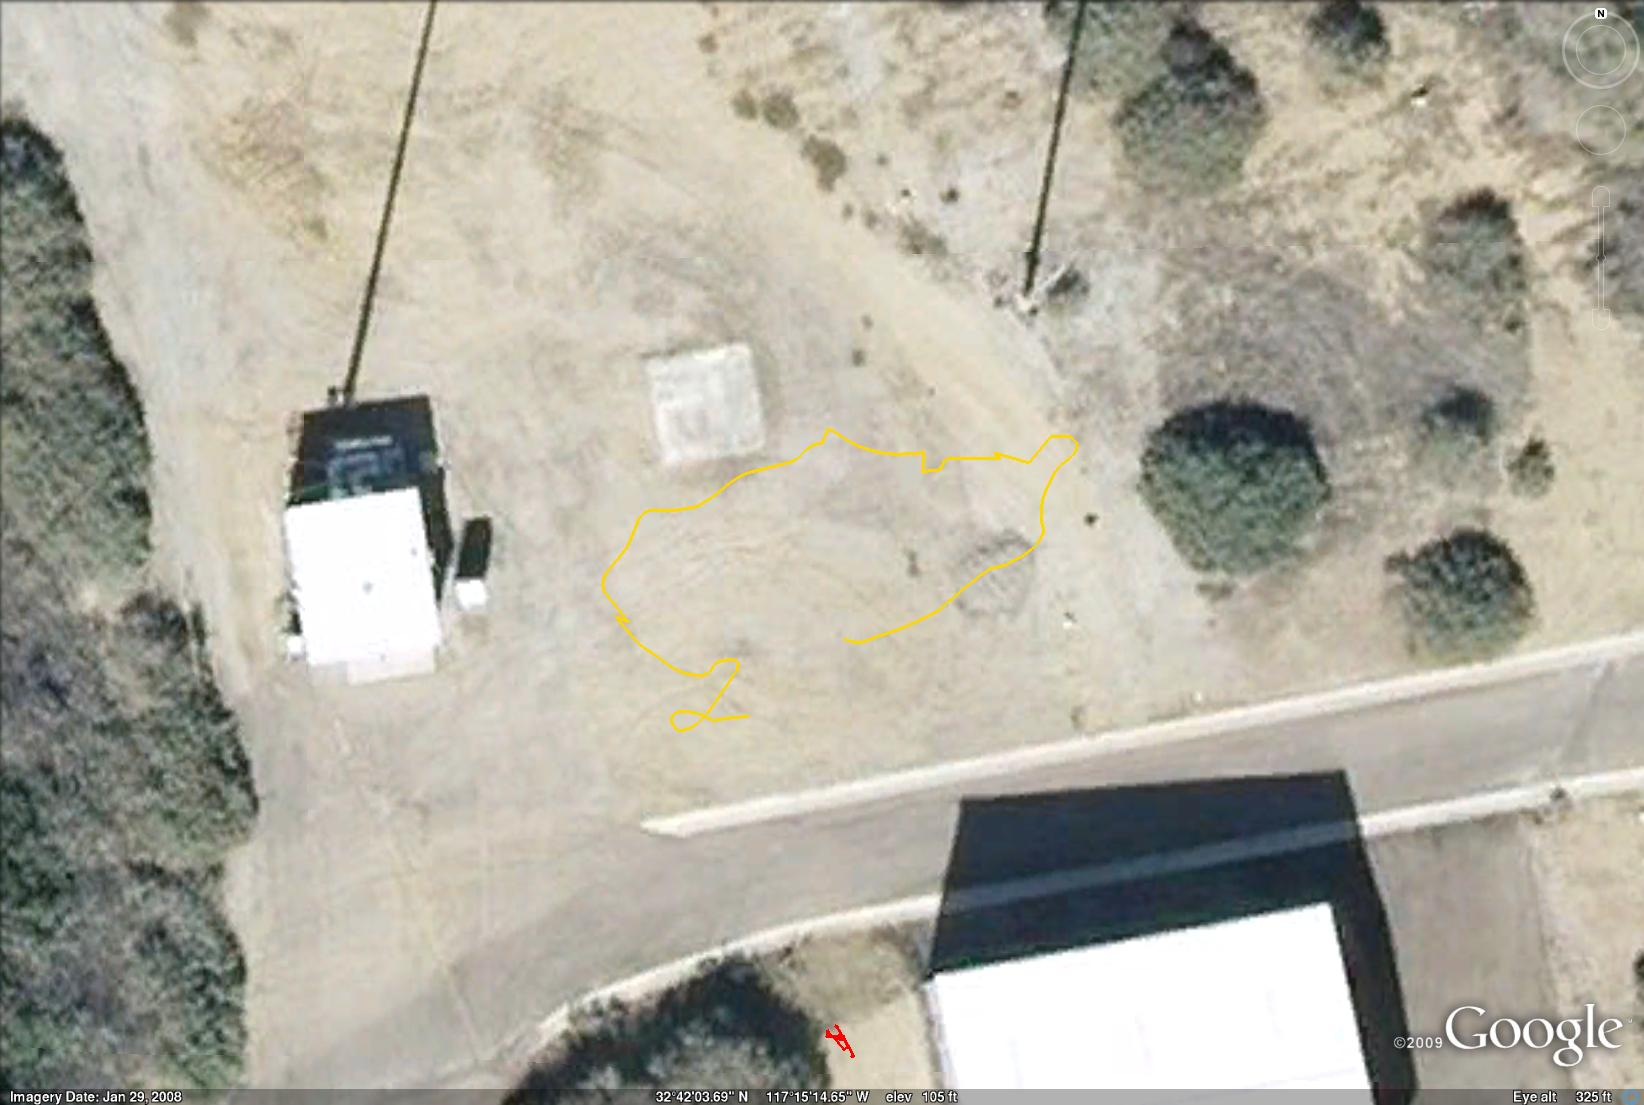
\includegraphics[width=.95\textwidth]{images/kfPlainDataFirstAttempt}
	\caption{Kalman filter output using the default parameters. The robot track is shown in yellow and a static GPS receiver with DGPS corrections is shown in red.}
	\label{fig:kfPlainDataFirstAttempt}
\end{figure}

\section{Lyapunov Controller Results}
\label{sec:lyapunovResults}
The initial attempt at running the Lyapunov controller on the PackBot resulted in rather poor performance that was likely caused by either mismatched units or the wrong equations being used in the code (see Figure \ref{fig:lyapunovDataFirstAttempt}).

\begin{figure}[ht!]
	\centering
	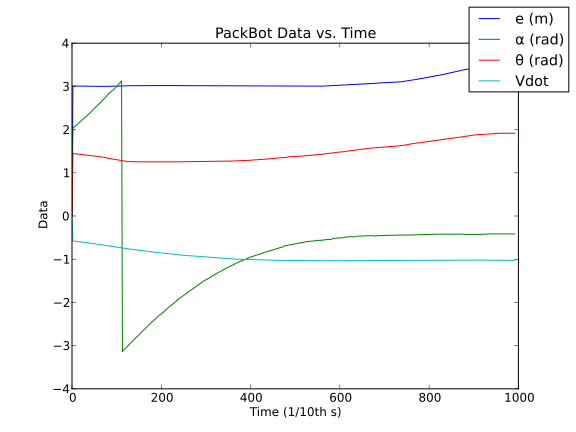
\includegraphics[width=.95\textwidth]{images/pbData}
	\caption{First attempt at running the PackBot using the Lyapunov controller.}
	\label{fig:lyapunovDataFirstAttempt}
\end{figure}